

\section{OpticalElement: \textquotedbl{}default\_ro\textquotedbl{}%
  \label{opticalelement-default-ro}%
}

\textbf{Element}: relay\_optics

\textbf{Alias}: RO

\textbf{Description}: Simple stand-alone relay optics module


\subsection{Global properties%
  \label{global-properties}%
}

\begin{quote}
\begin{alltt}
\begin{lstlisting}[frame=single]
 temperature : !ATMO.temperature
psf_filename : None
element_name : default_ro
\end{lstlisting}
\end{alltt}
\end{quote}


\subsection{Effects%
  \label{effects}%
}

Summary of Effects included in this optical element:

\setlength{\DUtablewidth}{\linewidth}
\begin{longtable*}[c]{|p{0.133\DUtablewidth}|p{0.226\DUtablewidth}|p{0.203\DUtablewidth}|p{0.110\DUtablewidth}|p{0.179\DUtablewidth}|}
\hline
\textbf{%
element
} & \textbf{%
name
} & \textbf{%
class
} & \textbf{%
included
} & \textbf{%
z\_orders
} \\
\hline
\endfirsthead
\hline
\textbf{%
element
} & \textbf{%
name
} & \textbf{%
class
} & \textbf{%
included
} & \textbf{%
z\_orders
} \\
\hline
\endhead
\multicolumn{5}{c}{\hfill ... continued on next page} \\
\endfoot
\endlastfoot

default\_ro
 & 
relay\_psf
 & 
FieldConstantPSF
 & 
True
 & 
{[}262, 662{]}
 \\
\hline

default\_ro
 & 
relay\_surface\_list
 & 
SurfaceList
 & 
True
 & 
{[}20, 120, 520{]}
 \\
\hline
\end{longtable*}
\label{tbl-default-ro}


\subsubsection{FieldConstantPSF: \textquotedbl{}relay\_psf\textquotedbl{}%
  \label{fieldconstantpsf-relay-psf}%
}

\textbf{Included by default}: \texttt{True}

\textbf{File Description}: SCAO PSF

\textbf{Class Description}: <no docstring>

\textbf{Changes}:

\begin{itemize}
\item \end{itemize}


\paragraph{Data%
  \label{data}%
}

\begin{figure}[H]
\noindent\makebox[\linewidth][c]{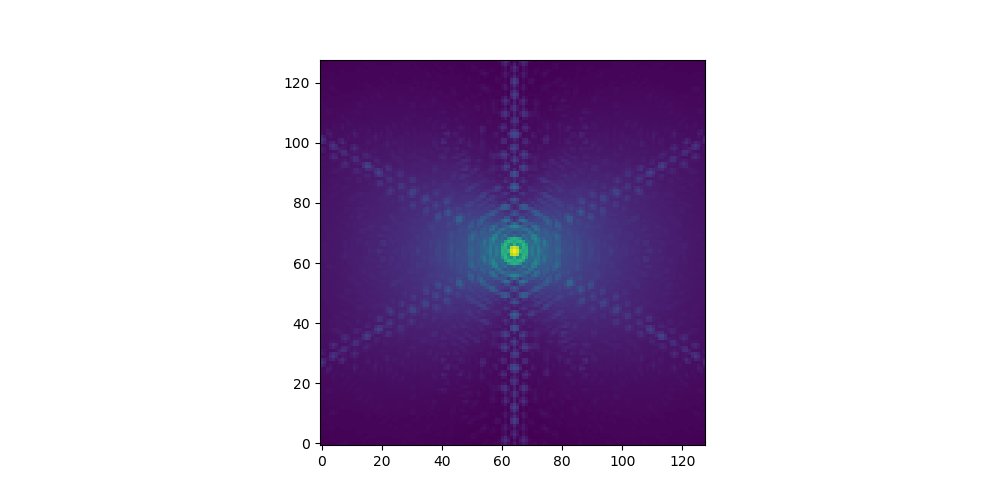
\includegraphics{relay_psf.png}}\phantomsection\label{fig-relay-psf}
\end{figure}


\paragraph{Meta-data%
  \label{meta-data}%
}

\begin{quote}
\begin{alltt}
\begin{lstlisting}[frame=single]
            filename : PSF_SCAO_ConstPSF_0_5off.fits
                name : relay_psf
         temperature : 7
        psf_filename : None
        element_name : default_ro
             warning : Default PSF is NOT field varying. See documentation.
              SIMPLE : True
              BITPIX : 8
               NAXIS : 0
              EXTEND : True
              AUTHOR : Kieran Leschinski
            DATE_CRE : 2019-07-30
            DATE_MOD : 2019-07-30
              SOURCE : AnisoCADO
              STATUS : Best guess for a standard observations
               ETYPE : CONSTPSF
                ECAT : -1
               EDATA : 1
             XOFFSET : 0
             YOFFSET : 5
             z_order : [262, 662]
             include : True
       flux_accuracy : 0.001
      sub_pixel_flag : False
       convolve_mode : full
            wave_key : WAVE0
    normalise_kernel : True
 report_plot_include : True
report_table_include : False
\end{lstlisting}
\end{alltt}
\end{quote}


\subsubsection{SurfaceList: \textquotedbl{}relay\_surface\_list\textquotedbl{}%
  \label{surfacelist-relay-surface-list}%
}

\textbf{Included by default}: \texttt{True}

\textbf{File Description}: list of surfaces in the relay optics

\textbf{Class Description}: <no docstring>

\textbf{Changes}:

\begin{itemize}
\item 2018-11-19 (KL) Added meta data

\item 2019-01-28 (KL) Fixed YAML format in meta data

\item 2020-07-18 (KL) Added all 6 mirrors from the CM16 update pdf

\item 2020-07-18 (KL) Pegged temperature to atmosphere
\end{itemize}


\paragraph{Data%
  \label{id1}%
}

\begin{figure}[H]
\noindent\makebox[\linewidth][c]{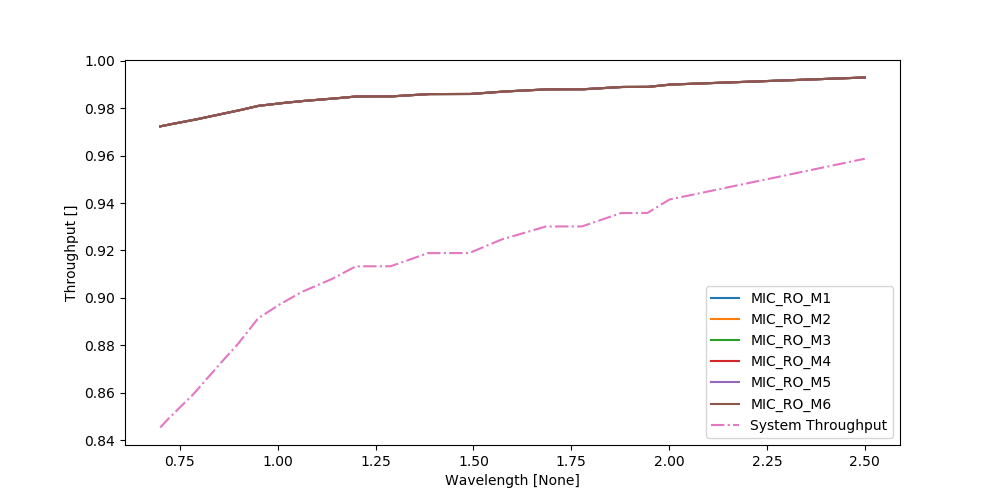
\includegraphics{relay_surface_list.png}}\phantomsection\label{fig-relay-surface-list}
\end{figure}

\setlength{\DUtablewidth}{\linewidth}
\begin{longtable*}[c]{|p{0.111\DUtablewidth}|p{0.068\DUtablewidth}|p{0.068\DUtablewidth}|p{0.068\DUtablewidth}|p{0.195\DUtablewidth}|p{0.121\DUtablewidth}|p{0.333\DUtablewidth}|}
\hline
\textbf{%
name
} & \textbf{%
outer
} & \textbf{%
inner
} & \textbf{%
angle
} & \textbf{%
temperature
} & \textbf{%
action
} & \textbf{%
filename
} \\
\hline
\endfirsthead
\hline
\textbf{%
name
} & \textbf{%
outer
} & \textbf{%
inner
} & \textbf{%
angle
} & \textbf{%
temperature
} & \textbf{%
action
} & \textbf{%
filename
} \\
\hline
\endhead
\multicolumn{7}{c}{\hfill ... continued on next page} \\
\endfoot
\endlastfoot

MIC\_RO\_M1
 & 
0.505
 & 
0.0
 & 
45.0
 & 
!ATMO.temperature
 & 
reflection
 & 
TER\_MICADO\_mirror\_mgf2agal.dat
 \\
\hline

MIC\_RO\_M2
 & 
0.51
 & 
0.0
 & 
10.0
 & 
!ATMO.temperature
 & 
reflection
 & 
TER\_MICADO\_mirror\_mgf2agal.dat
 \\
\hline

MIC\_RO\_M3
 & 
0.184
 & 
0.0
 & 
10.0
 & 
!ATMO.temperature
 & 
reflection
 & 
TER\_MICADO\_mirror\_mgf2agal.dat
 \\
\hline

MIC\_RO\_M4
 & 
0.53
 & 
0.0
 & 
10.0
 & 
!ATMO.temperature
 & 
reflection
 & 
TER\_MICADO\_mirror\_mgf2agal.dat
 \\
\hline

MIC\_RO\_M5
 & 
0.406
 & 
0.0
 & 
20.0
 & 
!ATMO.temperature
 & 
reflection
 & 
TER\_MICADO\_mirror\_mgf2agal.dat
 \\
\hline

MIC\_RO\_M6
 & 
0.406
 & 
0.0
 & 
35.0
 & 
!ATMO.temperature
 & 
reflection
 & 
TER\_MICADO\_mirror\_mgf2agal.dat
 \\
\hline
\end{longtable*}
\label{tbl-relay-surface-list}


\paragraph{Meta-data%
  \label{id2}%
}

\begin{quote}
\begin{alltt}
\begin{lstlisting}[frame=single]
            filename : LIST_RO_SCAO_mirrors.dat
                name : relay_surface_list
         temperature : !ATMO.temperature
        psf_filename : None
        element_name : default_ro
              author : Oliver Czoske, Kieran Leschinski
              source : P12_RelayOptics_Status_2020-06-23-MICADO-CM16-RO-v2.pdf
        date_created : 2018-11-19
       date_modified : 2020-08-17
              status : Design, pre FDR list of stand-alone SCAO relay optics mirrors
                type : mirror:list
          outer_unit : m
          inner_unit : m
          angle_unit : degree
    temperature_unit : deg_C
             z_order : [20, 120, 520]
             include : True
        ignore_wings : False
            wave_min : !SIM.spectral.wave_min
            wave_max : !SIM.spectral.wave_max
           wave_unit : !SIM.spectral.wave_unit
            wave_bin : !SIM.spectral.spectral_resolution
 report_plot_include : True
report_table_include : True
  minimum_throughput : !SIM.spectral.minimum_throughput
             etendue : !TEL.etendue
\end{lstlisting}
\end{alltt}
\end{quote}
